\documentclass[12pt,onecolumn,a4paper]{article}
\usepackage{epsfig,graphicx,amsthm,amsmath}
\usepackage{color,xcolor}
\usepackage{pgfplots}
\pgfplotsset{compat=newest}
\usepackage{tikz}
\usepackage{caption}
\usepackage{subcaption}
\usepackage{xepersian}
\settextfont{XB Zar}
\setlatintextfont{Times New Roman}

\newtheorem{theorem}{قضیه}[section]
\newtheorem{corollary}{نتیجه‌}[theorem]

\pgfplotstableread[col sep = comma]{gibbs.csv}\gibbs
\pgfplotstableread{
-1 0
-1 -1
0 -1
0 1
1 1
1 0
}\gibbsref

\begin{document}
\title{توجیه وجود مثال‌های خصمانه \\ و انتقال‌پذیری آن‌ها} 
\author{رامین براتی}
\date{\today}
\maketitle

\begin{abstract}
چکیده
\end{abstract}

\section{مقدمه} 
مقدمه.

\section{کارهای مرتبط}
دیدگاه پاکت‌های نادر.
دیدگاه خطی بودن.
دیدگاه کج کردن مرز.

\section{پدیده‌ی رونگه و مثال‌های خصمانه}
در این بخش، دیدگاه جدیدی را در مورد دلیل وجود مثال‌های خصمانه و انتقال‌پذیری آن‌ها ارائه می‌دهیم. در این دیدگاه، مثال‌های خصمانه را اثر جانبی پدیده‌ی رونگه دانسته و انتقال‌پذیری آن‌ها را با استفاده از اصل داربو توجیه می‌کنیم. ابتدا پدیده‌ی رونگه را توصیف می‌کنیم. در آنالیز عددی، پدیده‌ی رونگه مشکلی است که هنگام درون‌یابی با استفاده از چندجمله‌ای‌های درجه بالا به وجود می‌آید. طبق قضیه‌ی تقریب وایرشتراس\LTRfootnote{Weierstrass approximation theorem}،
هر تابع پیوسته‌ی 
$f(x)$
که بر روی یک بازه‌ی
$[a,b]$
تعریف شود را می‌توان با استفاده از یک چندجمله‌ای درون‌یاب
$P_n(x)$
تقریب زد. به عبارت دقیق‌تر
\begin{equation*}
    \lim_{n\rightarrow \infty}\left(\max _{{a\leq x\leq b}}\left|f(x)-P_{n}(x)\right|\right)=0.
\end{equation*}
طبق این قضیه، طبیعی است که انتظار داشته باشیم که با افزایش 
$n$
به تقریب دقیق‌تری از تابع مورد نظر دست یابیم. با این وجود، ممکن است که چندجمله‌ای‌هایی که انتخاب شده‌اند خاصیت همگرایی یکپارچه را نداشته باشند. توجه کنید که قضیه‌ی تقریب وایرشتراس فقط وجود این چندجمله‌ای را تضمین می‌کند، و مسیری برای یافتن این چندجمله‌ای مشخص نمی‌کند. در واقع، چندجمله‌ای‌هایی که به این صورت ساخته می‌شوند ممکن است با افزایش درجه‌ی چندجمله‌ای واگرا شوند. این مشکل به صورت الگوهای نوسانی بروز کرده که در نزدیکی نقاط درون‌یابی انتهایی بازه افزایش می‌یابد. شناسایی این پدیده را به  کارل رونگه
\LTRfootnote{Carl David Tolme Runge}،
ریاضیدان آلمانی، منتصب می‌کنند.

تابع رونگه با تعریف 
$f(x)=\frac{1}{1+25x^2}$ 
را در نظر بگیرید. چندجمله‌ای درون‌یاب این تابع را با استفاده از نقاط 
$x_i$ 
تعریف می‌کنیم، به طوری که
$x_{i}=\frac{2i}{n}-1$ 
و 
$i\in \left\{0,1,\dots ,n\right\}$.
همان گونه که مشاهده می‌شود، نقاط 
$x_i$ 
در بازه‌ی 
$[-1,1]$ 
و با فاصله‌ی یکسان توزیع شده‌اند. رونگه متوجه شد که چندجمله‌ای درون‌یابی که به روش ذکر شده ساخته شود، در نزدیکی مرز‌های دامنه‌ی تابع نوسان می‌کند. حتی می‌توان نشان داد که خطای درون‌یابی با افزایش 
$n$ 
 به صورت بیکران افرایش می‌یابد.

پدیده‌ی رونگه هنگام درون‌یابی با استفاده از پایه‌های تک‌جمله‌ای\LTRfootnote{Monomial basis} 
بروز پیدا می‌کند. با این حال تغییر این توابع پایه برای حل مسئله کافی نیست. اگر از توابع پایه‌ی مثلثاتی، مثلا توابع پایه‌ی چبیشف، برای تشکیل چندجمله‌ای درون‌یاب استفاده کنیم، با مشکل مشابهی مواجه می‌شویم. این مشکل  با نام پدیده‌ی گیبس\LTRfootnote{Gibbs phenomenon}
شناخته می‌شود. پدیده‌ی گیبس باعث به وجود آمدن نوساناتی در نزدیکی ناپیوستگی‌های سیگنال ورودی شده و این امر موجب فراجهش
\LTRfootnote{overshoot} 
در این نقاط می‌شود. در شکل 
\ref{fig:runge_gibbs} 
این دو پدیده با مثال‌هایی نشان داده‌ شده‌اند.

 \begin{figure}
    \centering
    \begin{subfigure}[b]{0.45\textwidth}
        \centering
        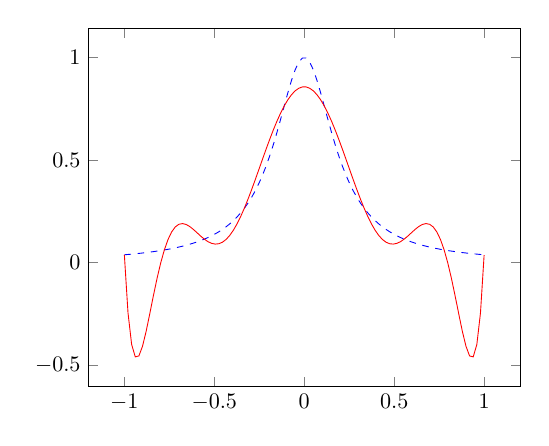
\begin{tikzpicture}[scale=0.8]
            \begin{axis}[xmin=-1,xmax=1,xmin=-1.2,xmax=1.2,samples=100]
                \addplot[domain=-1:1,blue,dashed]{1/(1+25*x*x)};
                \addplot[domain=-1:1,red,solid]{16.545674722429712 * x*x*x*x*x*x*x*x*x*x + 8.851286807773627e-13 * x*x*x*x*x*x*x*x*x + -12.079377458718012 * x*x*x*x*x*x*x*x + -1.6319051537287015e-12 * x*x*x*x*x*x*x + -22.778903788331114 * x*x*x*x*x*x + 8.747268893200492e-13 * x*x*x*x*x + 25.348331583973515 * x*x*x*x + -1.4087385060936399e-13 * x*x*x + -7.854564043148674 * x*x + 6.6005027351349585e-15 * x + 0.8573005222561162};
            \end{axis}
         \end{tikzpicture}
        \caption{پدیده‌ی رونگه}
        \label{fig:runge}
    \end{subfigure}
    \hfill
    \begin{subfigure}[b]{0.45\textwidth}
        \centering
        \begin{tikzpicture}[scale=0.8]
            \begin{axis}[xmin=-1,xmax=1,xmin=-1.2,xmax=1.2,samples=100]
                \addplot[mark=none,blue,dashed] table{\gibbsref};
                \addplot[mark=none,red,solid] table{\gibbs};
            \end{axis}
         \end{tikzpicture}
        \caption{پدیده‌ی گیبس}
        \label{fig:gibbs}
    \end{subfigure}
       \caption{دو پدیده‌ی رونگه و گیبس. در هر دو نمودار خم آبی تابع هدف و خم قرمز تقریب متناظر با آن تابع می‌باشد. (آ) تابع رونگه و تقریب آن توسط یک چندجمله‌ای درجه 10. (ب) تابع پله‌ای و تقریب آن با استفاده از 30 جمله‌ی اول سری فوریه‌ی متناظر آن.}
       \label{fig:runge_gibbs}
\end{figure}

همان گونه که در شکل نیز مشاهده می‌شود، پدیده‌ی رونگه تاثیر به مراتب مخرب‌تری از پدیده‌ی گیبس دارد. در واقع، می‌توان نشان داد که خطای درون‌یابی  در مثال بالا برابر با 
$O(2^n‌)$ 
است، در حالی که خطایی که پدیده‌ی گیبس در محاسبات وارد می‌کند 
$O(1)$ 
است.

با توجه به اینکه بهبود مشاهده شده بدون تغییر در تابع هدف، روش آموزش یا تغییر فاکتور غیرخطی حاصل شده، دور از ذهن نیست که انتقال‌پذیری مثال‌های خصمانه حاصل از اصل داربو باشد. ابتدا اصل داربو را آن طور که در (کتاب) آمده بیان می‌کنیم.
\begin{theorem}[اصل داربو]
    در تمامی انواع بسط طیفی (از جمله سری‌های توانی عادی)، هم دامنه‌ی همگرایی در صفحه مختلط و هم نرخ همگرایی توسط مکان و قدرت بدترین تکینگی در صفحه‌ی مختلط تعیین می‌شود. در اینجا، منظور از تکینگی قطب‌ها، توان‌های کسری، لوگاریتم‌ها و دیگر نقاط شاخه و ناپیوستگی‌های تابع 
    $f(z)$ 
    یا هرکدام از مشتقات آن است.
\end{theorem}

از اصل داربو می‌توان قضیه‌ی فرعی زیر را مستقیما نتیجه گرفت.

\begin{corollary}
    اگر دو تابع 
    $f(z)$ 
    و 
    $g(z)$ 
    دارای تکینگی‌های یکسان محدود کننده‌ی همگرایی باشند، ضرایب مجانب بسط طیفی آن‌ها در حد
    $n \rightarrow \infty$ 
    برابر خواهد بود.
\end{corollary}

همان گونه که در (مقاله) ذکر شده است، مثال‌های خصمانه‌ی یک شبکه را می‌توان به شبکه‌ی دیگری که بر روی داده‌های آموزشی متفاوتی آموزش داده شده است منتقل کرد. با توجه به نتیجه‌ی مستقیم اصل داربو، انتقال‌پذیری مثال‌های خصمانه را می‌توان به وجود تکینگی‌ها در تابعی که قصد یادگیری آن را داریم نسبت داد. این موضوع توجیه قابل قبولی برای انتقال مثال‌های خصمانه بین شبکه‌های مختلف، که مستقل از داده‌های آموزشی استفاده شده است، ارائه می‌دهد. حال تعاریف لازم برای تشریح دلیل وجود مثال‌های خصمانه، چگونگی تاثیر آن‌ها بر خروجی شبکه و انتقال‌پذیری آن‌ها را داریم.

مثال‌های خصمانه نقاطی در همسایگی مثال‌های طبیعی در نزدیکی مرز دامنه‌ی ورودی شبکه هستند که خروجی شبکه در همسایگی این مثال‌ها نوسنات شدیدی ناشی از پدیده‌ی رونگه دارد. در نتیجه، با استفاده از اطلاعات گرادیان تابع در آن نقطه، می‌توان نقطه‌ی دیگری در همسایگی آن مثال طبیعی یافت که شبکه با اطمینان بالایی آن را اشتباه طبقه‌بندی می‌کند.

به عبارت دیگر، اکثر مثال‌های طبیعی در نزدیکی یا روی مرز دامنه‌ی ورودی هستند\footnote{به عنوان مثال، در 
\lr{MNIST} 
اکثر ابعاد ورودی مقدار ۰ یا ۱ را دارند که دقیقا بر روی مرز دامنه‌ی ورودی قرار گرفته است.}
و محدوده‌ی همگرایی بسط طیفی یادگیری شده در این نقاط بسیار کوچک است و با کمی جابه‌جایی می‌توان از این محدوده خارج شد. این مسئله، احتمالا در ابعاد بالا بسیار تشدید می‌شود، زیرا در ابعاد بالا اکثر جرم فضا در نوار نازکی اطراف مرز دامنه‌ی ورودی قرار گرفته است. با توجه به این موضوع، بسیار محتمل است که وجود اختلالات خصمانه‌ی جهانی، که در (مقاله) مطرح شده‌اند، ناشی از این توزیع شدن مثال‌های طبیعی در نزدیک مرزها باشد.
\section{نتایج}
نتایج.

\end{document}